\chapter{Designing and Implementing SmartFin Combinators} \label{combinators-main}

The top-level representation of SmartFin financial contracts by a generic smart contract has been described already in chapter \ref{smart-contract-impl}, but the actual semantics of each combinator must also be represented in this smart contract. This chapter describes how the semantics of SmartFin's combinators are implemented. The modules covered in this chapter are displayed in figure \ref{fig:combinator-block} as a dependency graph. \\

\begin{figure}[h]
    \centering
    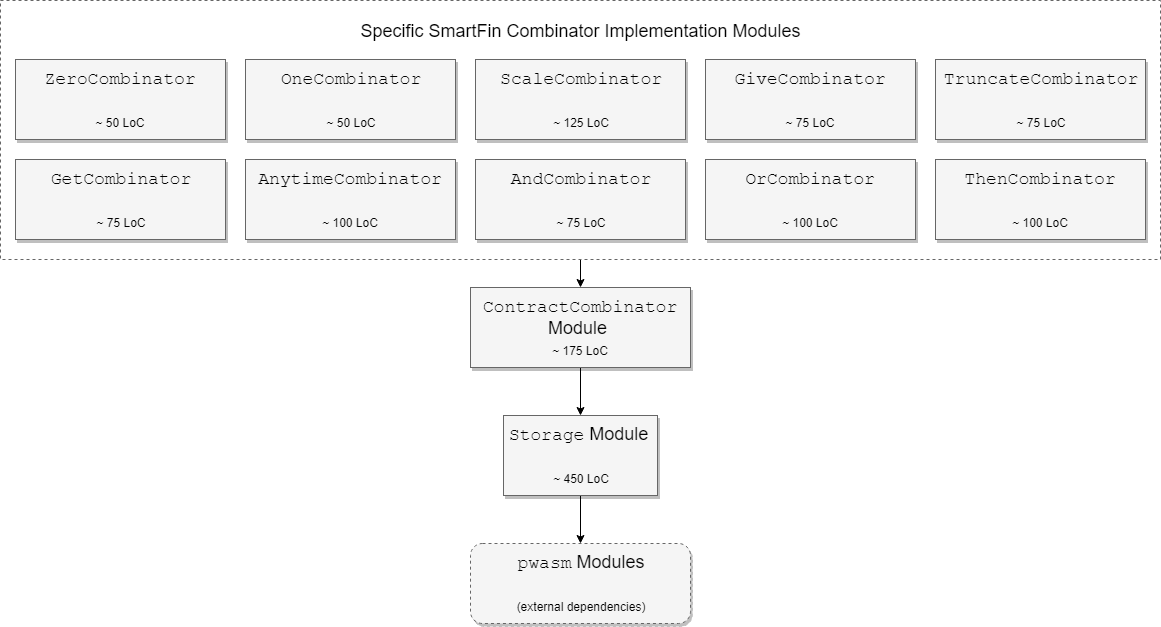
\includegraphics[width=\textwidth]{combinator-block.png}
    \caption{A dependency graph of the modules implemented to represent the SmartFin combinator semantics, with their approximate \textit{Lines of Code} (not including tests). \texttt{pwasm} modules are external dependencies, described in section \ref{smart-contract-tech}. The \texttt{Storage} module is described in section \ref{storage}.}
    \label{fig:combinator-block}
\end{figure}


\section{Designing a Programmatic Representation of SmartFin Combinators} \label{combinators-design}

\subsection{General Representation of Combinators}

As described in chapter \ref{combinator-DSL}, SmartFin is functional and compositional by definition. In any proposed smart contract implementation of SmartFin, representing the combinators in a functional manner is not simple; the smart contract must keep track of state over time, and individual combinators will have different state to keep track of. This suggests that a purely functional representation of the combinator behaviour may not be ideal, as keeping track of state could be complicated and unwieldy. \\

Furthermore, each combinator's functionality cannot be described simply as a single function - for example, how can we represent the \texttt{get} combinator, which acquires its sub-combinator at its horizon, without scheduled callbacks (which aren't possible within Ethereum smart contracts)? It makes more sense to represent it with an acquisition function and an \texttt{update} function which is called at a later date. \\

Due to the requirements of keeping track of state, and declaring multiple functions over this state, it would make sense to represent the combinators as classes rather than functions. As such, each combinator has a struct and a trait implementation. Due to the modular nature of the combinators in SmartFin, the information each combinator requires about their sub-combinators is minimal - there are no cases where certain combinations of combinators have non-standard behaviour. Because of this, the combinators implement a standard trait (\texttt{ContractCombinator}) for their functionality. \\

While the combinators cannot be easily represented in a smart contract in a functional manner, this does \textit{not} mean that they cannot be represented in a \textit{compositional} manner. In SmartFin, combinators may have a number of sub-combinators; this can represented as a tree of combinator objects, where each object may have zero, one, or two sub-combinator objects. This would be simpler than using some other data structure (e.g. a vector) to store the combinators, as it removes any extra requirements of external knowledge; each combinator object will only know about its sub-combinator objects, and nothing else. It also makes logic for traversal by recursion simple, intuitive, and efficient. \\

In summary, the final design for the representation of SmartFin's combinators in the smart contract is a tree of objects. Each object is a struct which implements the \texttt{ContractCombinator} trait, allowing combinators to call methods on sub-combinators without knowing which combinators they represent. Each combinator will store its own sub-combinators in its struct, and method calls will be propagated by recursive calls to the sub-combinators. Each combinator's behaviour will be implemented entirely within its struct's method implementations. \\

To illustrate this idea, take the SmartFin version of the financial contract representing a European option from section \ref{example-contracts}, \texttt{get truncate <01/01/2020 00:00:00> or scale 500 one zero}; the representation of these combinators as a tree of struct instances is depicted in figure \ref{fig:euro-option-tree}. \\

\begin{figure}[h]
    \centering
    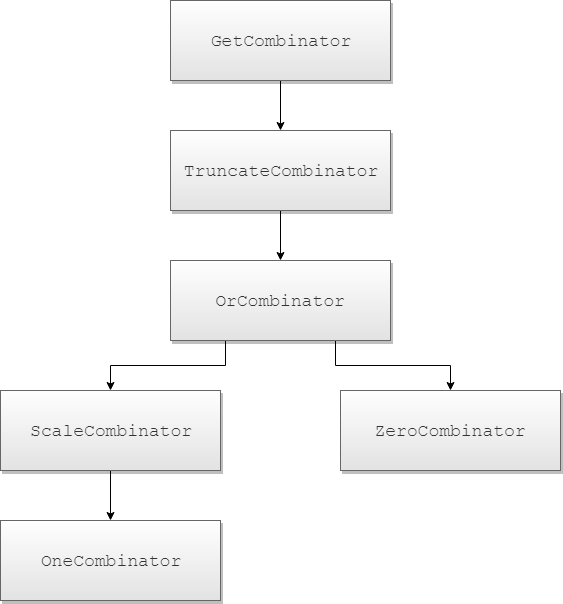
\includegraphics[width=0.7\textwidth]{euro-option-tree.png}
    \caption{The representation of the European option SmartFin contract, \texttt{truncate <01/01/2020 00:00:00> or scale 500 one zero}, as a tree of combinator struct instances.}
    \label{fig:euro-option-tree}
\end{figure}


\subsection{\texttt{ContractCombinator} Methods} \label{contract-combinator-trait}

The \texttt{ContractCombinator} trait is a trait that all combinator structs implement, with methods that are required regardless of the combinator type. This enables combinators to call methods on their sub-combinators regardless of the sub-combinators' types, and the same for the top-level smart contract. These methods are as follows: \\

\begin{itemize}
    \item \texttt{get\_horizon}: returns the combinator's horizon as an \texttt{Option<u32>}, with the value \texttt{Some(<U\-NIX Epoch time>)} if a horizon exists, or \texttt{None} otherwise.
    \item \texttt{past\_horizon}: returns true if the given time (in UNIX Epoch time) is beyond the combinator's horizon.
    \item \texttt{acquire}: handles the acquisition of the combinator (and sub-combinators if applicable).
    \item \texttt{update}: handles updating the combinator to the current time, mainly to evaluate payments that occur since the last call to \texttt{update}. The method returns the amount of funds in Ether that the counter-party should have paid the holder in this period, as a signed 64-bit integer (where a negative result signals payments from the holder to the counter-party).
    \item \texttt{get\_combinator\_number}: returns the combinator's enum value.
    \item \texttt{get\_combinator\_details}: returns a \texttt{CombinatorDetails} struct, containing the combinator's acquisition time as an \texttt{Option<u32>}, and whether or not it has been fully-updated as a \texttt{bool} (i.e. further calls to \texttt{update} will have no effect). These details can be used by parent combinators, or by the top-level smart contract - i.e. to check if the contract has concluded or been acquired.
    \item \texttt{serialize}: returns the combinator (and sub-combinators) in a serialized format (\texttt{Vec<i64>}), which is required to store the combinator tree in smart contract storage.
    \item \texttt{serialize\_details}: returns the combinator's \texttt{CombinatorDetails} struct in a serialized format (\texttt{Vec<i64>}), which is called when serializing the combinator. This is a trait method to provide a general implementation of this method, given that the \texttt{CombinatorDetails} objects have the same structure regardless of the combinator type, and all combinators implement the \texttt{get\_combinator\_details} method. \\
\end{itemize}

Besides these trait methods, each struct implementing \texttt{ContractCombinator} also implements a \texttt{deserialize} constructor. These are not present in the \texttt{ContractCombinator} trait because they are static - as there is no combinator object until after deserialization - and static methods cannot be defined for traits in Rust. This method takes in a vector representing the combinator tree, with all of its state, in a serialized format. It also takes in an index, which is the location of the combinator being deserialized in the vector. The method returns the deserialized \texttt{ContractCombinator} instance and the last index used during deserialization. The index is needed for combinators like \texttt{and}, where the starting index of the second sub-combinator is not known until the first sub-combinator is deserialized.


\section{Implementation} \label{combinator-implementation}

Every combinator has their own struct and implementation of the \texttt{ContractCombinator} trait, and the \texttt{ContractCombinator} module has some extra functionality for utility.


\subsection{The \texttt{ContractCombinator} Module}

The \texttt{ContractCombinator} module defines default implementations of some methods for the \linebreak\texttt{ContractCombinator} trait, as well as some utility methods.


\subsubsection{Default Method Implementations for the \texttt{ContractCombinator} Trait}

Default implementations are not provided for the \texttt{acquire}, \texttt{update}, and \texttt{get\_combinator\_number}, as these implementations obviously depend entirely on which combinator is being implemented. A default \texttt{get\_combinator\_details} method is also not implemented, as there is no way to declare that structs will have a specific member variable when implementing a trait (as opposed to something like a Superclass in other languages). As such, there is no way to obtain the \texttt{ContractDetails} struct from the member variable as far as the \texttt{ContractCombinator} trait is aware, and so each combinator struct must implement their own method to retrieve this variable. This is a specific limitation with Rust. In all combinators, the methods \texttt{get\_combinator\_number} and \texttt{get\_combinator\_details} have a trivial implementation, and so they are not mentioned further. \\

The default \texttt{get\_horizon} implementation returns \texttt{None}, as any combinators without sub-combina\-tors will have no horizon, and so it is the basest implementation of the method where no extra information about the combinator type is required. The default \texttt{past\_horizon} implementation gets the horizon with \texttt{get\_horizon}; if the horizon is \texttt{None}, then the horizon can never be passed, otherwise it is compared to the given time. This is never overridden by any \texttt{ContractCombinator} implementations, as it will never change as long as \texttt{get\_horizon} is accurate. \\

The default \texttt{serialize\_details} implementation pushes the combinator enum, the acquisition time (represented as the value, or -1 if no value exists), and whether or not the combinator is fully-updated (1 represents \texttt{true}, 0 represents \texttt{false}). These are obtained by the \texttt{get\_combinator\_number} and \texttt{get\_combinator\_details} functions. This is standard for all combinators, and is used in the \texttt{serialize} method. \\

The \texttt{serialize} method is required to store the combinator and its state in the smart contract storage between function calls, and serializes this information into a vector of signed 64-bit integers (or \texttt{i64}s). The default implementation of this method simply returns the return value of \texttt{serialize\_details}; this will represent any combinators with no extra state, and the other combinators will have to serialize their own state.


\subsubsection{Other Utilities in the \texttt{ContractCombinator} Module}

Besides the trait implementation, the \texttt{ContractCombinator} module also provides several utilities. One such utility is a \texttt{Combinator} enum representing the contract combinators defined in chapter \ref{combinator-DSL}, and implementations for converting between this enum and an integer (for serialization purposes). \\

The \texttt{CombinatorDetails} struct definition is also provided here, containing the acquisition time of a combinator, and whether or not a combinator is fully-updated. All combinators are able to return their \texttt{CombinatorDetails} struct; \texttt{fully\_updated} is used to prevent calling into combinators for no reason, and \texttt{acquisition\_time} is used to ensure that combinators have been acquired (especially \texttt{anytime} combinators) before being called into. Two methods for initialising a \texttt{CombinatorDetails} struct are also provided, one with default attributes (no acquisition time and not fully-updated), and one from the serialized format of the \texttt{CombinatorContract} struct. \\

The \texttt{ContractCombinator} module also provides two public functions for comparing times; \texttt{earliest\_time} will take in two times and return the value of the earliest, and \texttt{latest\_time} will take in two times and return the value of the latest. \\

The module also provides a function for deserializing combinators - given a serialized combinator vector and a starting index, the function will check the serialized combinator's enum and initialise a combinator object of the correct type using the correct \texttt{deserialize} constructor.


\subsection{Simple \texttt{ContractCombinator} Implementations}

Several of the \texttt{ContractCombinator} implementations have simple implementations throughout all of the combinator modules. The \texttt{get\_combinator\_number} method returns the value in the \texttt{Combinator} enum representing the implementing combinator's type. The \texttt{get\_combinator\_details} method just returns the \texttt{CombinatorDetails} object from struct. \\

\texttt{get\_horizon} typically returns \texttt{None}, or the latest horizon of any sub-combinators (except in the case of \texttt{truncate}). \texttt{serialize} will write the result of \texttt{serialize\_details} to a vector, followed by any struct variables, and then any sub-combinators sequentially. While it isn't on the trait, all combinators have a \texttt{deserialize} function which reads from a serialized vector as described and reconstructs the combinator struct. \\

Besides these methods, all combinators implement their own \texttt{acquire} and \texttt{update} methods as described below. All of these \texttt{acquire} methods will throw an error if the combinator is previously acquired or expired, and the \texttt{update} methods will return 0 balance change if the combinator is not acquired in the past or is fully updated.


\subsection{The \texttt{ZeroCombinator} and \texttt{OneCombinator} Modules}

The \texttt{acquire} method for both the \texttt{ZeroCombinator} and \texttt{OneCombinator}'s implementations of \texttt{ContractCombinator} both set the combinator's acquisition time to the current time. For the \texttt{update} method, both combinators mark themselves as fully-updated, \texttt{ZeroCombinator} returns 0 as the evaluated difference in balances, and \texttt{OneCombinator} returns 1.


\subsection{The \texttt{AndCombinator} Module}

The \texttt{acquire} method for the \texttt{AndCombinator} checks if the sub-combinators' horizons have passed yet. For each sub-combinator, if the horizon has not passed then its \texttt{acquire} method is called with the same parameters as the \texttt{AndCombinator}'s. The \texttt{AndCombinator}'s acquisition time is then set to the current time. \\

The \texttt{update} method calls \texttt{update} on the two sub-combinators in order. If both of the two sub-combinators are fully-updated after their \texttt{update} calls, then the \texttt{AndCombinator} is set as fully-updated. The sum of the values returned by the sub-combinators is returned.


\subsection{The \texttt{OrCombinator} Module}

The \texttt{OrCombinator} struct is one of the more complicated combinator implementations, requiring the holder to select which of its two sub-combinators should be acquired. The struct contains the combinator's \texttt{or} index. This is the index of the \texttt{or} combinator in the combinator contract, with regard to all \texttt{or} combinators, ordered sequentially by left-to-right occurrence and starting from 0. This is used to index into a vector of all \texttt{or} combinator choices in the contract, stored in the \texttt{Storage} struct described in section \ref{storage}. \\

A method \texttt{get\_or\_choice} is provided on the struct, which determines which sub-combinator should be acquired when the \texttt{or} combinator is acquired. The result is represented by an \texttt{Option<bool>} value, where \texttt{Some(true)} represents the first sub-combinator, \texttt{Some(false)} the second, and \texttt{None} that neither sub-combinator should be acquired. If either sub-combinator is expired, a value signalling that the other should be acquired is returned. If neither is expired, the \texttt{or} choice is looked up and returned from storage. \\

The \texttt{acquire} uses \texttt{get\_or\_choice} to check which sub-combinator to acquire. If \texttt{Some(val)} is returned then the relevant sub-combinator's \texttt{acquire} method is called and the \texttt{OrCombinator}'s acquisition time is set to the current time, otherwise nothing occurs. \\

The \texttt{update} method obtains the \texttt{or} choice by calling \texttt{get\_or\_choice} with the \texttt{OrCombinator} instance's \textit{acquisition} time, \textit{not the current time}. If the sub-combinator to have acquired is ambiguous, the method returns 0. If a concrete \texttt{or} choice is returned, the method checks if the relevant sub-combinator has been acquired; if not, then its \texttt{acquire} method is called with the \texttt{OrCombinator}'s \textit{acquisition} time. After this check, the \texttt{update} method on the relevant sub-combinator is called and returned, and the \texttt{OrCombinator} is set to fully-updated if the relevant sub-combinator is also fully-updated.


\subsection{The \texttt{GiveCombinator} Module}

The \texttt{acquire} method simply acquires the sub-combinator and sets the acquisition time. \texttt{update} simply updates the sub-combinator and returns the negated result. The combinator's fully-updated flag is set to the value of the sub-combinator's fully-updated flag.


\subsection{The \texttt{ScaleCombinator} Module}

The \texttt{ScaleCombinator} is one of the more complicated combinator implementations. This is because a \texttt{scale} combinator scales the sub-contract's value by an observable. This observable can be a fixed constant, or it can be a value that varies over time. Both cases must be handled by this combinator. The \texttt{ScaleCombinator} struct has a scale value, an \texttt{Option<i64>} that represents the \texttt{scale} combinator's observable when it is a constant value.  The struct also has an observable index, an \texttt{Option<usize>} representing the \texttt{scale} combinator's observable's index in a set of time-varying observable values. One of the scale value or observable index must have a concrete value, i.e. \texttt{Some(v)}, and the other must have no concrete value, i.e. \texttt{None}. \\

The method \texttt{get\_scale\_value} is implemented on the \texttt{ScaleCombinator} struct. This method checks if a concrete scale value exists; if so, it is returned, otherwise the observable index is looked up through the \texttt{Storage} struct and returned (as an \texttt{Option<i64>} which may not yet have a concrete value). If neither a concrete scale value or observable index exists, an error is thrown. \\

The \texttt{acquire} method is simple, simply acquiring the sub-combinator and setting the acquisition time. The \texttt{update} method gets the scale value using \texttt{get\_scale\_value}. If no concrete scale value exists yet then the value 0 is returned, otherwise the sub-combinator is updated, and fully-updated is set if the sub-combinator is fully-updated. The sub-combinator's update value is then multiplied by the scale value and returned.


\subsection{The \texttt{TruncateCombinator} Module}

The \texttt{CombinatorContract} implementation for the \texttt{get\_horizon} implementation returns the earliest of the \texttt{TruncateCombinator}'s truncated horizon and the sub-combinator's horizon - as described in section \ref{DSL-semantics}. The \texttt{acquire} method simply checks the horizon as usual, acquires the sub-combinator, and sets the acquisition time. \texttt{update} performs the usual call-through to the sub-combinator, setting fully-updated to the sub-combinator's fully-updated value and returning the result from \texttt{update} on the sub-combinator.


\subsection{The \texttt{ThenCombinator} Module}

The \texttt{acquire} method checks if the current time is past the first sub-combinator's horizon. If not, the first sub-combinator is acquired, otherwise the second is acquired, and then the acquisition time is set. The \texttt{update} method checks if the \texttt{ThenCombinator}'s acquisition time is past the first sub-combinator's horizon (as before). If not, the first sub-combinator is updated, otherwise the second is updated. Fully-updated is then set based on the sub-combinator, and the sub-combinator's update value is returned.


\subsection{The \texttt{GetCombinator} Module}

The \texttt{GetCombinator} struct is another relatively simple \texttt{ContractCombinator} struct, although it may seem unintuitive at first. The \texttt{acquire} method carries out the main behaviour of the \texttt{get} combinator. The sub-combinator's horizon is checked, and if a concrete horizon is found then the sub-combinator is acquired \textit{with the horizon as the acquisition time}. This will cause the sub-combinator to only become updated once the horizon is reached or passed, as is required by the definition of the \texttt{get} combinator in section \ref{DSL-semantics}. The \texttt{update} method is simple, calling through to the sub-combinator and setting fully-updated and returning the sub-combinator's \texttt{update} result as usual.


\subsection{The \texttt{AnytimeCombinator} Module}

The \texttt{AnytimeCombinator} is one of the more complex combinators, allowing the acquisition of the sub-combinator at any point until its horizon (as described in section \ref{DSL-semantics}). The \texttt{AnytimeCombinator} struct has an \texttt{anytime} index. This is the index of this \texttt{anytime} combinator's sub-contract acquisition time, in a vector of \texttt{anytime} acquisition times stored in smart contract storage. \\

The vector contains \texttt{(bool, Option<u32>)} tuples - the boolean value represents whether or not the corresponding \texttt{anytime} combinator has been acquired, and the \texttt{Option<u32>} represents the prospective acquisition time of the sub-combinator. If this time is in the future, it can be changed by calling the \texttt{acquire\_anytime\_sub\_contract} method on the smart contract's ABI, setting it to the current time as long as the parent \texttt{anytime} combinator has been acquired. If the prospective acquisition time is in the past, then it cannot be changed. \\

The \texttt{acquire} method sets the \texttt{AnytimeCombinator}'s acquisition time and sets the prospective acquisition time of the sub-combinator in the stored \texttt{anytime} acquisition times vector to the sub-combinator's horizon. This means that the sub-combinator can be acquired manually up until its horizon, after which its acquisition time will be locked in as the horizon. We cannot call \texttt{acquire} in this method on the sub-combinator, as a combinator can only be acquired once and the sub-contract's acquisition time may change in the future. \\

The \texttt{update} method checks if the sub-contract has been acquired yet. If not, then the \texttt{anytime} acquisition times vector is checked for its prospective acquisition time. If the sub-combinator's acquisition time has passed then \texttt{acquire} is called on it. After this, \texttt{update} calls through to the sub-combinator as usual.


\section{Evaluation} \label{combinators-eval}

In order to evaluate the representation of the SmartFin combinators in the implemented smart contract, the design of the combinators' representation in the smart contract can be qualitatively evaluated, and automated testing can provide some quantitative evaluation of their correctness.


\subsection{Combinator Representation}

Representing the combinators as a tree of \texttt{ContractCombinator} structs results in an intuitive composition of combinators that behave as one would expect based on the SmartFin contract definition. Combinators apply behaviours over their sub-combinators, and then call through to the sub-combinators; a financial contract written in SmartFin would also apply behaviour and propagate acquisition to sub-combinators, and so this representation is a natural fit. \\

One potential implementation approach that may also seem like a natural fit is the implementation of each combinator as its own smart contract. This would allow a SmartFin contract written to be represented as a set of linked smart contracts. Calling methods on each smart contract would call through to the sub-combinator's smart contract. This may seem like a closer match to SmartFin's semantics, as any financial smart contracts would be able to become sub-contracts for other financial smart contracts. There are a few issues with this design, however. One issue is that either state would have to be replicated across every smart contract (e.g. the holder and counter-party address), or it would have to be passed across smart contract boundaries with every function call, which would become difficult to implement in a trustworthy manner (e.g. verifying that the holder is correct). Another issue is that traditional financial contracts are a "package deal" - either you acquire the whole contract, or none of it. Representing each combinator as a smart contract could make it difficult to prevent any combinator in the financial contract being acquired without its parents. Circumventing this would require some path representing the parent-child relationship between combinators to be marked through the smart contracts, somewhat defeating the purpose of this representation. Gas costs of deploying large financial smart contracts would also be much higher with multiple smart contracts. For these reasons, using a single smart contract to represent a SmartFin contract is preferable.


\subsection{Design of the \texttt{ContractCombinator} Trait}

On the whole, the design of the \texttt{ContractCombinator} trait facilitated the operation of the combinators fairly well, and the chosen methods make contract acquisition/updating simple in general. The ability to get a combinator's horizon, or check if a time is past its horizon, is effectively used by every combinator with sub-combinators; as such, the \texttt{get\_horizon} and \texttt{past\_horizon} methods are a useful part of the trait. The ability to serialize combinators relatively painlessly with \texttt{serialize\_details} and the guaranteed \texttt{serialize} method allowed the serialization of the combinators to operate intuitively and efficiently through recursion. Unfortunately, the trait did not provide such methods for deserialization as there can be no static methods defined on a trait. As such, the \texttt{deserialize} constructor was implemented on each combinator struct - this is a limitation of Rust. \\

Another slight issue with the \texttt{ContractCombinator} trait is the \texttt{get\_combinator\_details} and \texttt{get\_combinator\_number} methods. Every combinator has an implementation of these methods, despite the fact that the implementations are extremely similar. Both of these methods could be implemented on the \texttt{ContractCombinator} trait easily if there were a way to require the \texttt{ContractCombinator}-implementing structs to have certain member variables (like a Superclass); unfortunately, Rust does not provide such a mechanism, and so every struct must implement a method for this. Both methods are required to obtain information needed for serialization and for acquisition/updating the contract, so the current solution is currently the best option available in Rust. \\

Some possible changes that could be made to \texttt{ContractCombinator} involve defining more getter functions, including a function that would return a vector of sub-combinators (which would have 0, 1, or 2 elements). This would allow default implementations of many of the simpler methods in the \texttt{ContractCombinator} trait which typically call through to the sub-combinators, e.g. \texttt{get\_horizon} and \texttt{serialize}. Overall, this could potentially reduce the amount of repeated code required between the combinator implementations. Unfortunately, as mentioned already, there is no way to require the definition of a member variable on a struct implementing a trait in Rust. This means that instead of writing repeated implementations for \texttt{get\_horizon} and other simple methods, there would be more repetition of these getter functions. Unless some method of requiring struct members is implemented in Rust, the benefits to such a change would thus be minimal, hence why they went unimplemented. \\

While the recursive behaviour of the \texttt{acquire} method is a natural fit for the combinators, one possible issue with this design is that the expected behaviour of acquiring the SmartFin combinators has been split across two different methods - \texttt{acquire} and \texttt{update}. For example, typically acquiring the \texttt{one} combinator would result in a payment occurring from the counter-party to the holder; with the current implementation, acquiring the \texttt{one} combinator records no payments until \texttt{update} is called. This is more of a ramification of the design of the smart contract ABI than a direct design decision; the \texttt{update} method is implemented to keep track of payments over time, whereas the \texttt{acquire} method simply exists to denote acquisition times. Furthermore, the smart contract ABI updates the balance of the contract in its \texttt{acquire} method, nullifying this issue from any external point-of-view. Besides this, the need for an \texttt{update} method is obvious given the lack of scheduled callbacks/persistent operation of the smart contract, as explained in section \ref{contract-design}. These reasons justify the compromise of separate \texttt{acquire} and \texttt{update} methods.


\subsection{Design of the Combinators' Implementations}

Most of the combinators implement fairly trivial or straightforward behaviour, and as such there is little to discuss regarding their design. \\

The decided-upon implementation of the setting of observables' values is somewhat interesting. Due to the nature of Ethereum smart contracts, it is impossible to read observables' values from off-chain data. As such, the only way to obtain these values is to have them passed into the contract by an external user, or obtained from another smart contract (eventually requiring external user input). \\

In the definition of the original DSL by Peyton Jones et al.\cite{SPJ}, an observable is defined as something with a value that both the holder and counter-party would agree upon. This definition was considered for the setting of observables, leading to a design where both parties would need to provide a matching value for an observable to set its value. After a discussion with Dr. Panos Parpas of Imperial College London, who wrote financial contracts professionally in the past, this design was passed over in favour of letting a pre-defined arbiter set the value of an observable. This more closely matches the way that traditional financial contracts handle observables, where typically a pre-defined information source for the value of any observable will be included in the financial contract. This also prevents parties from lying about observable values to avoid unfavourable transactions - although, as described in \ref{contract-design}, it is impossible to bind the parties to a smart contract's terms without external tools.


\subsection{Testing}

In order to ensure that the combinator implementations behave correctly, extensive unit testing has been implemented to test the functionality of all structs implementing \texttt{ContractCombinator}. The tests follow the same structure for all combinators, but some combinators require extra tests. In total, there are 151 unit tests for the combinator modules, made up of ~2750 LoC. Besides the unit tests mentioned here, all combinators are tested in the Rust and JavaScript integration tests mentioned in section \ref{contract-testing}.


\subsubsection{\texttt{ContractCombinator} Module Tests}

The \texttt{ContractCombinator} module provided several utilities, for which unit tests have been written. The default implementations of the \texttt{ContractCombinator} methods were tested by implementing a \texttt{DummyCombinator} struct, which only implements methods with no default implementation. \\

The two time comparison methods, \texttt{earliest\_time} and \texttt{latest\_time}, are both tested with concrete values and \texttt{None} values for time. The methods for converting between the \texttt{Combinator} enum and integer values is tested for all of the enum values. The \texttt{serialize\_details} method is tested on the \texttt{DummyCombinator}, as well as the \texttt{serialize} implementation. The \texttt{deserialize\_combinator} method is tested by defining a combinator tree with all combinator types present and random state, and serializing it. This serialized tree is then deserialized and serialized again; if the second serialized vector is equal to the first, then the deserialization method works correctly - assuming that the serialization methods work correctly. The \texttt{deserialize_combinator} function is also tested with an empty serialized combinator vector, to ensure that the correct error is thrown.


\subsubsection{General Combinator Testing Methodology}

All of the combinators are unit-tested, mostly following the same testing methodology. For each combinator, the \texttt{get\_combinator\_number} and \texttt{get\_horizon} methods are tested. For combinators with sub-combinators, all variations of sub-combinator horizons are tested, e.g. first sub-combinator's horizon is later, second is later, both are undefined, etc. \\

The \texttt{acquire} method is also checked to ensure that it sets the \texttt{CombinatorDetails} struct's acquisition time member correctly, and \texttt{update} is checked to ensure that the struct's fully-updated flag is set when required. The value returned by calling \texttt{acquire} and then \texttt{update} is checked in all permutations (e.g. expired, non-expired, one sub-combinator expired, etc.). The \texttt{update} method is tested before \texttt{acquire} is called, or before the acquisition time is reached, to ensure that it does nothing. \\

The \texttt{serialize} method is testing by ensuring that all relevant information is encoded in the serialized combinator vector, where the combinator implements extra serialization beyond the default implementation. The \texttt{deserialize} constructor is tested by serializing, deserializing, and re-serializing the combinator (as with the \texttt{ContractCombinator} tests). Any errors which should be thrown are also tested. This covers the basic operation of all combinators, and only a few combinators require extra testing beyond this.


\subsubsection{Specific Combinator Tests}

The \texttt{OrCombinator} implementation is tested with the left and right sub-combinators chosen or expired for every testing scenario, as well as several tests where no choice is made yet. The implementation is also tested to ensure that behaviour remains consistent, i.e. you cannot choose one sub-combinator and then see the results of the other sub-combinator after updating. \\

The \texttt{ScaleCombinator} implementation is tested with constant scale values, defined observables, and undefined observables. It is also tested without either is set, to ensure that an error is thrown. \\

The \texttt{AnytimeCombinator} implementation is tested to ensure that acquisition of the sub-combinator occurs on calls to \texttt{update}, and that this is set to the horizon correctly. The \texttt{update} method is also tested by simulating acquisition of the \texttt{anytime} sub-contract, to ensure that it is acquired at the correct time, and that the value returned is correct. Tests with various combinations of acquisition and updating are implemented to ensure correctness and consistency of the acquisition/payment evaluation behaviour. It is also checked that the \texttt{AnytimeCombinator} throws the correct error when the \texttt{anytime} sub-contract acquisition time is before the parent \texttt{AnytimeCombinator}'s acquisition time.


\subsection{Conclusion}

Overall, the combinators' behaviour seems to follow the specification described in section \ref{DSL-semantics} based on the thorough unit and integration testing. The design is relatively representative of the SmartFin combinators, although some compromises had to be made due to the nature of smart contracts (like separate \texttt{acquire} and \texttt{update} methods). The design of the \texttt{ContractCombinator} trait covers all of the required functionality, and allows combinator implementations to be relatively simple on the whole.


\section{Remarks}

This chapter has described how SmartFin's combinators are represented in the implemented smart contract. The final result of this and the previous chapters is a smart contract implementation which can represent any given SmartFin contract, with minimal concessions made due to the nature of smart contracts. \\

While this is useful, we are still missing easy ways of creating, deploying, evaluating, and interacting with financial smart contracts; the next chapter will describe the web client created for this purpose.

